% %%%%%%%%%%%%%%%%%%%%%%%%%%%%%%%%%%%%%%%%%%%%%%%%%%%%%%%%%%%%%%%%%%%%%%%%%%%%%%%
% 2345678901234567890123456789012345678901234567890123456789012345678901234567890
% 1         2         3         4         5         6         7         8

%\documentclass[letterpaper, 10 pt, conference]{ieeeconf}  % Comment this line out
                                                          % if you need a4paper
\documentclass[a4paper, 10pt, conference]{ieeeconf}     % Use this line for a4
                                                          % paper

\IEEEoverridecommandlockouts                              % This command is only
                                                          % needed if you want
                                                          % to use the \thanks
                                                          % command
\overrideIEEEmargins
% See the \addtolength command later in the file to balance the column lengths
% on the last page of the document



% The following packages can be found on http:\\www.ctan.org
\usepackage{graphics} % for pdf, bitmapped graphics files
\usepackage{epsfig} % for postscript graphics files
\usepackage{mathptmx} % assumes new font selection scheme installed
\usepackage{times} % assumes new font selection scheme installed
\usepackage{amsmath} % assumes amsmath package installed
\usepackage{amssymb}  % assumes amsmath package installed

\usepackage{multirow}
\usepackage{graphicx}
\usepackage{amsmath}

\title{\LARGE \bf A Teleoperation System For Mobile Social Robots: Improving Operator Performance through Automatic Gaze Control and 3D Visualizations of Spatial Relationships}
%Other titles: 
%A Teleoperation System For Mobile Social Robots: Improving Customer Satisfaction through Autonomy and representation of 3D spatial relationships
%A GUI for Improving Customer Satisfaction (HRI) during the Teleoperation of Mobile Social Robots

\author{
\alignauthor Andres Mora \hspace{1cm} Dylan F. Glas \hspace{1cm} Takayuki Kanda\hspace{1cm} Norihito Hagita\\
\email{\{andresmora, dylan, kanda, hagita\}@atr.jp}
\thanks{A.~Mora, D.~F.~Glas, T.~Kanda and N.~Hagita are with Advanced Telecommunications Research Institute International, 2-2-2 Hikaridai, Keihanna Science City, Kyoto, Japan, 619-0288}\\
}

\begin{document}


\maketitle

\thispagestyle{empty}
\pagestyle{empty}


% %%%%%%%%%%%%%%%%%%%%%%%%%%%%%%%%%%%%%%%%%%%%%%%%%%%%%%%%%%%%%%%%%%%%%%%%%%%%%%%
\begin{abstract}
%%%ORIGINAL%%%
% The teleoperation of mobile social robots requires human operators to understand
% facial gestures and other non-verbal communication in order to facilitate an
% improved human-robot interaction. For more natural human-robot interactions and
% considering the current state-of-the-art, the operator should be provided with a
% system that incorporates mechanisms that shared-autonomy. In this paper, the
% authors identify requirements for a teleoperation system that are important for
% social human-robot interaction. Two techniques to satisfy these requirements are
% proposed: a 3D visualization of the robot's environment, and an autonomous
% control of the robot�fs gaze to keep a person within its field of view. A
% scenario where a robot plays the role of a shopkeeper was used to demonstrate
% that these techniques improve the quality of the interaction and decrease the
% operator's workload. Results from the conducted study show that the combination
% of the visualization of spatial relationships and the proposed automatic gaze
% control improves the teleoperation of the robot and consequently, customer
% satisfaction.

% Mobile social robotics is the field of robotics that deals with interacting with humans in everyday environments such as malls, eldery care centers, museums, etc.
% Currently, artificial intelligence, speech recognition and other technologies have not reached a level of reliability which would enable robots to be completely autonomous in these situations.
%In this paper, the authors identify unique requirements for the teleoperation of mobile social robots and developed a teleoperation system that allowed to examine their effects in a human-robot interaction.
% In this paper, the authors identified unique requirements for the teleoperation of mobile social robots and developed a novel 3D-based graphical user interface that allowed the examination of their effects in a human-robot interaction.
% In particular, the teleoperation of mobile social robots requires operators to understand facial gestures and other non-verbal communication of the person interacting with the robot, in order to facilitate an improved human-robot interaction.
% It is thus critical to provide the operators with tools that increase their comprehension of such communication and of the physical environment in which the robot is situated.
% % The authors demonstrate the importance and effectiveness of an automatic control of the robot's gaze to follow a customer's face, as long as it is combined with an appropriate representation of the spatial relationships of the environment where the interaction takes place.
% A study where a robot plays the role of a shopkeeper was conducted to demonstrate that when the operator is freed from following a customer's face using our proposed automatic control of the robot's gaze, undesirable side effects occurred, such as operators getting disoriented and navigation becoming inaccurate.
% In order to solve the problems caused by these side effects, the authors developed a graphical user interface which combines a 3D representation of the spatial relationships of the simulated shop with the designed automatic gaze control.
% The results of this study demonstrated that providing the operator with the implemented representations of the spatial relationships reduced undesirable side effects of our automatic gaze control, its benefits were maintained and the quality of the interaction with the customer was improved.


% Teleoperation is, therefore, an important methodology to understand the intentions, facial expressions and gestures of the person interacting with the robot and achieve smooth, natural human-robot interactions.
% It then becomes critical to provide the operators with tools that increase their understanding of the context and the environment in which the robot is involved.
% In this paper, a study where a robot plays the role of a shopkeeper was conducted.
% This study showed that when the operator is freed from routine tasks (in our case, follow a customer's face using an automatic control of the robot's gaze), unexpected side effects occurred, e.g. operators got disoriented and navigation became inaccurate.
% It was demonstrated, however, that when the operator was given a 3D representation of the spatial relationships of the simulated shop in addition to the automatic gaze control, these side effects were solved and the quality of the interaction with the customer improved.


%Friday25.02.11
% The teleoperation of mobile social robots requires operators to understand facial gestures and other non-verbal communication of the person the robot is interacting with, in order to facilitate an improved human-robot interaction. 
% To achieve smooth, natural human-robot interactions it is critical to provide the operators with tools that increase their understanding of the context and the environment in which the robot is involved.
% In this paper, the authors demonstrate the importance and effectiveness of introducing shared-autonomy in a teleoperated system, as long as it is combined with an appropriate representation of the spatial relationships of the environment where the interaction takes place. 
% % an autonomous control of the robot's gaze to keep a person within its field of view during a human-robot interaction, as long as it is combined with a representation of the spatial relationships in the environment.
% A study where a robot plays the role of a shopkeeper was conducted to validate the following concept.
% The combination of an autonomous control of the robot's gaze to keep a person within its field of view and the 3D representation of the spatial relationships has a stronger positive impact on the quality of the human-robot interaction and on decreasing the operator's workload than by applying them independently.
% Therefore, the combination of these factors improves the teleoperation of a mobile social robot and consequently, customer satisfaction.

%Results from the conducted study show that the combination of these factors improves the teleoperation of the robot and consequently, customer satisfaction.
 
% In this paper, the authors explore the requirements for a teleoperation system for social human-robot interaction.
% From these requirements, the authors analyze the effects of a 3D visualization of the robot's environment, and an autonomous control of the robot�fs gaze to keep a person within its field of view during a human-robot interaction. 
% A study where a robot plays the role of a shopkeeper was conducted to demonstrate that the combination of these factors has a stronger positive impact on the quality of the interaction and on decreasing the operator's workload than by applying them independently.
% Results from the conducted study show that the combination of the visualization of spatial relationships and an automatic gaze control improves the teleoperation of the robot and consequently, customer satisfaction.

The teleoperation of mobile social robots requires operators to understand facial gestures and other non-verbal communication of the person interacting with the robot.
It is also critical for the operator to comprehend the surrounding environment, in order to facilitate an improved human-robot interaction.
%It is thus critical to provide the operators with tools that increase their comprehension of such communication and of the physical environment in which the robot is situated.
%However, the task of providing this information to the opertor is not trivial. 
%Although allowing the operator to control where the robot looks to obtain a visual feedback of the person interacting with the robot can help the operator observe non-verbal communication, it can also produce undesirable side effects, such as operators getting disoriented and navigation becoming inaccurate.
Allowing the operator to control where the robot looks to obtain visual feedback of the person interacting with the robot can help the operator observe non-verbal communication. 
However, it can also produce undesirable side effects, such as operators getting disoriented and navigation becoming inaccurate.
%In order to solve the problems caused by these side effects, the authors developed a graphical user interface which combines an automatic gaze control of the robot's gaze and  a 3D representation of the spatial relationships of the simulated shop.
In order to solve the problems caused by these side effects, the authors developed a graphical user interface which combines an automatic control of the robot’s gaze and a 3D representation of the surrounding environment, such as location of items and configuration of a shop.
A study where a robot plays the role of a shopkeeper was conducted to validate the proposed GUI.
It was demonstrated that when providing the operator with the implemented representations of the spatial relationships, the benefits of the proposed automatic gaze control were maintained, the undesirable side effects were reduced, and the quality of the interaction with the customer was improved.


\end{abstract}

%%%%%%%%%%%%%%%%%%%%%%%%%%%%%%%%%%%%%%%%%%%%%%%%%%%%%%%%%%%%%%%%%%%%%%%%%%%%%%%%
\section{Introduction}
% The quest for a ``natural'' interaction with a human is what strongly motivates the development of new methodologies and technologies in the field of social human-robot interaction (HRI).
% 
% Due to limitations in today's artificial intelligence and recognition technologies, full automation of social robots will not be possible for some time.
% However, these limitations can be bypassed by using an person operating the robot (from now on referred to as operator) to perform certain recognition and decision-making tasks. 

Mobile social robotics is the field of robotics that deals with interacting with humans in everyday environments such as malls, elderly care centers, museums, etc.
Currently, artificial intelligence, speech recognition and other technologies have not reached a level of reliability which would enable robots to be completely autonomous in these situations.

Using teleoperation to augment partial autonomy is not only useful for laboratory studies (using Wizard-of-Oz (WOZ) methods \cite{green:applying, steinfeld:theOz, dahlback:wizard}) but will also be valuable in actual deployments of social robots in commercial applications for safety and legal reasons. 
The development of social robots which incorporate teleoperation brings together two very different branches of human-robot interaction (HRI). 
One is social HRI, which focuses on studying psychological aspects of conversational interactions between people (from now on referred to as {\it customers}) and robots.
The other is HRI for teleoperation, which typically focuses on issues like the workload of the {\it operator} (person remotely controlling the robot), situation awareness and shared autonomy for the remote operation of non-social robots.

%As these fields traditionally focus on very different problems, little research has explored the intersection between them, leaving many questions unanswered.
% How do teleoperation systems for social robots differ from those for traditional robots? 
%Little research has explored the intersection between these fields, leaving many questions unanswered.
Little research has explored different techniques for teleoperating mobile social robots, leaving many questions unanswered.
What new requirements exist for social robots? What new techniques can aid a teleoperator in controlling social robots effectively?


Keeping track of a person's face is fundamental for social interactions, yet, manually actuating this task requires a large amount of effort by the operator.
An automatic gaze control technique of the robot's head was implemented to keep the customer during our study within its field of view and relieve the operator from this routine task.

%Although our implemented automatic gaze control has benefits such as reducing the operator's actuation workload and increasing the operator's awareness of the customer's state, including facial expressions and gestures; the authors found it also has some drawbacks.
Although our implemented automatic gaze control has benefits such as reducing the operator's actuation workload and increasing the operator's awareness of the customer's state, including facial expressions and gestures; the authors found that the automatic gaze control has some drawbacks; it reduces the operator's awareness of surrounding environment, and makes an operator less effective in navigation.
% These drawbacks include an unintended disorienting side effect on the operator (given the operator's reduced awareness of the state of the robot) and thus could not use the video information effectively for navigational purposes.
These drawbacks include an unintended disorienting side effect on the operator which reduced the operator's awareness of the state of the robot and thus could not use the video information effectively for navigational purposes.
This reduced awareness is due to the increased attention the operator gives to the video presenting the customer's face which results in a lower understanding of the location and orientation of the robot within its environment, and the locations of objects and people around the robot.

To overcome this difficulty, a 3D graphical user interface (GUI) was created to represent the robot's environment which augments the operator's understanding of spatial relationships.
In this paper, we establish that a teleoperation system for mobile social robots must provide the operator with an appropriate representation of spatial relationships when automatic gaze control is used.
The authors conducted an experiment where a robot plays the role of a shopkeeper. 
The results of the experiment demonstrated that when this representation was present, the awareness issues were effectively tackled and the benefits of the proposed automatic gaze control were also retained.
% The results of an experiment where a robot plays the role of a shopkeeper, demonstrate that when this representation was present, the awareness issues were effectively tackled and in addition, the benefits of our proposed automatic gaze control were also retained.
In addition, when both factors are available, the operator can improve the quality of the human-robot interaction.

% In this paper, we establish that a teleoperation system for mobile social robots must provide the operator with an appropriate representation of spatial relationships when the operator uses our proposed automatic gaze control.
% In addition, when both factors are available, the operator can improve the quality of the human-robot interaction.

% In this paper, a fundamental requirement is established between an appropriate representation of the 3D spatial relationships of the environment where the human-robot interaction takes place and the use of our proposed automatic gaze control in a teleoperation system for mobile social robots.

% In order to answer these questions, the authors conducted preliminary experiments during which it was observed that the operators required constant help from the teleoperating system to carry out their tasks. 
% It was also noted however, that even if the operators were provided with such aid, they remained confused with regards to the location of the robot within the environment where the robot had the interaction with a ``customer''.  

% Increasing the autonomy of the robot should decrease the operator's workload.  However, this is often a trade-off, as increased autonomy can contribute to the "operator out of the loop" problem.  
% This leads to the operator having a reduced understanding of the state of the robot, and thus unable to operate it as effectively as when the robot is under full manual control.
% 
% The authors acknowledged that following the person's face was necessary for social interactions, but that manually actuating this required a large amount of effort.
% Therefore, the authors designed an automatic gaze control of the robot's head to keep the person interacting with the robot within its field of view. 
% This autonomous behavior accounts for benefits such as reducing the operator's actuation tasks and increasing the operator's awareness of the customer's state, including facial expressions and gestures. 
% However, this autonomous behavior does also have drawbacks, namely: the unintended side effect of disorienting the operator because the operator had a reduced awareness of the state of the robot, and thus could not use the video information effectively for navigational purposes. 
% Regarding the awareness that the operator loses includes the location and orientation of the robot within its environment, and the locations of objects and people around the robot. 
% To overcome these problems, the authors created a 3D representation of the robot's environment to augment the operator's understanding of these two factors.  
% 
% After conducting an experiment where a robot plays the role of a shopkeeper, the results demonstrate that when this representation was present, the awareness issues were effectively tackled, but also the benefits of our proposed automatic gaze control also retained. 
% 
% Therefore, the authors demonstrate that there is a fundamental link between an appropriate representation of the 3D spatial relationships and the use of our proposed automatic gaze control in a teleoperation system for mobile social robots. 

% In this paper, the authors provide a new understanding of the effect of combining shared autonomy with visual representations of spatial relationships for the teleoperation of mobile social robots.
% Shared autonomy is represented in our study by an automatic gaze control of the robot's head to keep the person interacting with the robot within its field of view.
% The visual representations of the spatial relationships in the environment where the interaction takes place are presented to the operator through a three-dimensional (3D) graphical user interface (GUI).
% 
% After conducting an experiment where a robot plays the role of a shopkeeper, the authors demonstrate that by introducing our proposed automatic gaze control, the quality of the human-robot interaction does increase.
% However, the improvement resulting from the combination of the shared autonomy and our 3D representation of spatial relationships had a greater positive impact on the interaction.
% Therefore, the authors demonstrate that there is a fundamental link between an appropriate representation of the spatial relationships and the use of shared autonomy in a teleoperation system for mobile social robots. 


% In this paper, our main goal is to identify and analyze the effect of various factors during the teleoperation of a mobile social robot. 
% These factors include both the presentation of information and the use of partial autonomy to assist the operator.
% In order to validate the effect of these factors a study where a robot plays the role of a shopkeeper was conducted. 
% The results of this study present how the combination of two factors (namely, the representation of spatial relationships and a proposed automatic gaze control) produce an improved human-robot interaction which was reflected by an increased customer satisfaction. 
% In addition, the results show that the independent effect of each of these factors do not amount for a similar enhancement of the interaction.

%In this paper, we identify several key requirements for teleoperation of social
%robots, and we present some new techniques based on a shared-autonomy approach
%which address these requirements.

% %%%%%%%%%%%%%%%%%%%%%%%%%%%%%%%%%%%%%%%%%%%%%%%%%%%%%%%%%%%%%%%%%%%%%%%%%%%%%%%
\section{Related Works}
\subsection{Teleoperation for navigation tasks}
For mobile robots that have to accomplish navigation tasks in order to carry out missions such as search and rescue, military tasks or space exploration, there are two opposite approaches along the ends of a spectrum: being completely teleoperated by humans \cite{burke:moonlight, wells:talon, yamauchi:packbot} or being fully automated \cite{buehler:darpa}. 
Some of the aspects of research on teleoperation involve increasing and maintaining the level of situational awareness of the operator\cite{drury:decomposition, drury:awareness}, combining mixed and virtual reality techniques to help the operator improve the navigation of the robot~\cite{carff:human}, and the design of the Graphical User Interface (GUI) to be used to remotely operate the robot.

Particular to the design of GUIs for navigational robots, a number of studies have been done regarding the way to present information~\cite{meier:sensorfusion, nielsen:comparing}. 
One notable finding could be summarized as the need to combine different types of information altogether~\cite{drury:lassoing, nielsen:ecological}. 
In specific, how does the navigation of the robot improve with a GUI that integrates a video feed and map data within a 3D environment, in contrast to video-based only or map-based only GUI.

%Although existing knowledge in this domain has proven useful, further understanding of the requirements in the field of HRI is imperative.
Although existing knowledge in this domain has proven useful, further understanding of the requirements governing the teleoperation of mobile social robots is imperative.
The teleoperation of social robots requires observation of new kinds of information (e.g. gestures, facial expressions, tone of voice, relative positioning) as well as to address new problems in actuation that may arise (controlling conversation, gaze direction, and gestures; following someone via locomotion or gaze control). 
Our approach to solve these issues are presented in later sections of this paper. 

\subsection{Teleoperation of social robots}
In practice, the WOZ methodology in HRI involves the remote control of a robot system. 
In that respect, it appears to be similar to teleoperation. 
However, the system that allows the operator to do so, is seen as a tool and not as a research topic in itself.

In the work carried out by Kuzuoka~\cite{kuzuoka:dual}, focus is given to the ``ecology'' among operators and customers. In this study the idea of the operator acquiring all the information through a video-only interface is conducted and no map information is provided. 
It reports the fact that what the operator utilizes (in this case, a three-screen based GUI) is not necessarily a good factor for the interaction with a customer e.g. due to the robot's lack of natural motion.

%In our study, the authors explore the display of other kinds of information to the operator, in addition to video-only interfaces as well as methods to liberate the operator from reiterative actuation tasks.

\subsection{Natural interaction with social robots}
In this study, our focus is to enable a ``context-sensitive'' interaction between a human and social robots, where the robots' interaction go beyond simple question-answer-type or command-receiving-type  interaction. 
In the scope of this paper, the importance is the adaptability of the robot to the customer's context, including a location, surrounding objects, attention, and subtle reaction (see our watch shop scenario in Section~\ref{sec:experiment} as an example of such interaction).
There are a number of studies with social robots conducted for natural interaction. 
There are many aspects to be studied, such as knowledge on non-verbal behaviors, like natural way of gazing \cite{carff:human, drury:lassoing}, proximity behavior \cite{drury:decomposition, drury:awareness}, the way of social dialog \cite{green:applying}, and social patterns \cite{woods:comparing}. 
These studies are certainly useful for future social robots; however, the context of users was often out of focus in this type of studies.
Some previous studies in robotics have aimed to recognize users' context, like a way to recognize joint attention behavior \cite{glas:simultaneous}, attention \cite{glas:field} and engagement \cite{glas:laser}. 
Although new techniques are constantly being developed, the robots' capabilities in context-sensitive interactions have remained highly limited.

%%%%%%%%%%%%%%%%%%%%%%%%%%%%%%%%%%%%%%%%%%%%%%%%%%%%%%%%%%%%%%%%%%%%%%%%%%%%%%%%
\section{Design Principles}
Previous work on the teleoperation of mobile robots has been mainly focused on navigational robots whereas little is known about the teleoperation of mobile social robots.
The basic design of our teleoperation system was created according to this previous knowledge on teleoperation for navigational robots. 
%Additional techniques for the teleoperation of social robots in particular are also proposed.
This section introduces the authors' proposed techniques for the teleoperation of mobile social robots and the guidelines on which these techniques are based on.

\subsection{Guidelines for Navigational Robotics}
Research on the teleoperation of mobile robots, using traditional 2D GUIs, has shown that distributing information on different locations of the interface may result in an increased workload and decreased performance of the operator \cite{nielsen:ecological}.
These results may be caused by poor situation awareness of the operator.
Situation awareness can be referred to as the level of understanding of the operator with respect to the environment around the robot that allows the operator to provide accurate instructions to the robot \cite{nofi:defining}.

In \cite{nielsen:comparing}, a study compares the usefulness of combining map and video information in a navigation task by comparing a side-by-side 2D representation and an integrated 3D representation. 
This study reports that the integration of map and video information in a 3D-based GUI positively affected the performance of the operator during navigation of the robot.
However, the scope of this study is only a navigational task and it does not addresses important issues such as observing facial gestures of a customer and how they would affect the performance of an operator. 
 
From a design perspective, Nielsen et al. \cite{nielsen:ecological} summarize that to improve situation awareness in human-robot systems it is recommended to: a) use a map, b) fuse sensor information, c) minimize the use of multiple windows and d) provide more spatial information to the operator. 
%Based on these recommendations, particularly on \cite{nielsen:comparing}, the authors have implemented a GUI that serves as a baseline to our study.
%This baseline incorporates laser range data, a video feed and a 3D model of the robot used in this research.
Based on these recommendations, the authors have implemented a GUI that incorporates laser range data, a video feed, a 3D model of the robot used in this research and a 3D representation of the environment where the robot is located.

\subsection{Proposed Techniques}
\label{subsec:proposed}
In addition to these guidelines, two fundamental mechanisms for facilitating the teleoperation of a mobile social robot are proposed: automatic gaze control and visualization of spatial relationships.
The first one helps relieve the operator from continuously having to direct the camera towards the customer and the second one helps the operator retain the awareness that may be lost by providing the operator with autonomy.
% In addition to these guidelines, the authors propose the combined use of two fundamental mechanisms for facilitating the teleoperation of a mobile social robot: automatic gaze control and visualization of spatial relationships.

\subsubsection{Automatic Gaze Control}
%The teleoperation of mobile social robots requires the operator to be capable of navigating the robot smoothly and safely through an environment, to identify people and obstacles and to be able to interact with them accordingly.
%A critical requirement for such system is to allow the operator to observe the facial expressions and gestures of the person interacting with the robot.
A critical requirement for the teleoperation of mobile social robots is to allow the operator to observe the facial expressions and gestures of the customer.
%Typically, this information is provided to the operator through a video feed; in this way, the operator can understand the intentions of the person interacting with the robot.
Typically, this information is provided to the operator as a video feed coming from a camera pointing to the object or location of interest; in this way, the operator can understand the intentions of the customer.
However, the actuation required by the operator to maintain the customer within the field of view of the robot's camera may increase the workload of the operator, especially when the customer may continuously move inside the environment.
 
% Another requirement is to allow the operator to keep track of people in the environment, particularly that one interacting with the robot. 
% People who interact with the robot may continuously move inside the environment.
% This behavior could become a large source of workload for the operator. 

Thus, the automation of such task would become useful to reduce the effect of this workload on the performance of the operator.
A feature called ``automatic gaze control'' is proposed to allow the system to automatically control the robot's gaze (i.e.\ camera direction) to follow a person's location and the person's face. 
The operator then, is able to observe the facial expressions and gestures of the person interacting with the robot without the tedious responsibility of maintaining the robot's gaze direction manually.
\begin{figure*}[htp] \centering
\includegraphics[width=2\columnwidth]{figs/fullFeatureGUIFinal_2.eps}
	\caption{GUI with the implemented visualization of spatial relationships and automatic gaze control}
	\label{fig:fullFeatureGUI}
\end{figure*}
% \vspace{-1mm}

\subsubsection{Visualization of Spatial Relationships}
The proposed automatic gaze control is intended to release the operator from continuously following a customer's face in order to decrease the workload in terms of actuation and allow the operator to easily concentrate on the customer's facial expressions.
However, this level of attention of the operator into the video feed may raise problems in the awareness of the operator, e.g. the location of static and dynamic objects in the areas of the environment not shown by the limited field of view of the video feed. 
% A video feed represents a natural way for operators to understand spatial relationships. 
% However, the narrow field of view that cameras provide may limit this understanding. 
In addition, if the robot is required to point at different objects and interact with multiple customers in the environment, the operator would need to actively observe their locations.
Relying solely on the video feed would force the operator to create a ``mental map'' to remember where several objects are in the environment \cite{dejong:improving}.

Therefore, it becomes essential to visualize spatial relationships between the robot and both static and dynamic objects in the environment. 
Using graphical visualization of such spatial relationships in conjunction with a video feed would increase the overall perception of the environment, by releasing the operator from the need to create a mental map of the objects in the environment, since they are represented on the GUI.

Through combination of the design recommendations presented in \cite{nielsen:comparing} with our proposed techniques, an enhanced robot control by the operator reflected in an improved human-robot interaction is expected.

%%%%%%%%%%%%%%%%%%%%%%%%%%%%%%%%%%%%%%%%%%%%%%%%%%%%%%%%%%%%%%%%%%%%%%%%%%%%%%%%
\section{System Implementation}
Given that our approach incorporates shared autonomy, implementation is necessary on both the robot side and operator side.
This section presents how the concepts of visualizing spatial relationships and automatic gaze control are carried out within the proposed teleoperation system. % Figure~\ref{fig:fullFeatureGUI}.


\subsection{Robot side}
\label{subsubsec:robotSide}
%The implemented system on the robot side consists of two major modules: the utilized robot and the human tracking module.
The robot testbed used in our research is called ``Robovie II''. 
It comprises a mobile base (Pioneer 3) and an upper body that has two arms, each with 4 degrees of freedom (DOF) and a head with 3DOF. 
The arms can be used to point at the objects of interest as well for other gestures that complement its utterances. 
The head has a camera, a microphone and a speaker to allow an operator to gather information about the environment and the person the robot is interacting with. 
Robovie has two laser range sensors attached to its mobile base (about 10$[cm]$ from the ground), one in the front and one in the back, in order to cover almost 360$[\deg]$ around the robot to detect obstacles.

The representation of people and their real-time position within the environment is based on the tracking data provided by a human tracker module. 
This module combines the range data from six SICK\copyright laser sensors located around the interaction environment. 
The human tracker module detects and tracks people using a technique that is based on the algorithm presented in \cite{glas:laser}. 
The estimation of the positions for a person is done by particle filters and a contour-analysis technique is used to estimate the direction in which a person is facing~\cite{glas:field}. 

\subsection{Operator Side}
The data gathered by the sensors onboard of Robovie and by the environmental sensory system (human tracker module) are presented to the operator through a 3D-based interface.

The proposed GUI combines the two factors discussed in Section~\ref{subsec:proposed}, and aims to allow the operator to identify and locate a person and objects of interest quickly, as well as to establish social distances accurately.
Figure~\ref{fig:fullFeatureGUI} shows an instance of the proposed system's GUI. The interface is divided in two sections: a visualization area (top) where a video feed is combined with a 3D model of the controlled robot and range data from laser sensors, and an actuation control area (bottom). 

%The main area presents fused information about the environment surrounding the robot and the robot itself at a low level. The laser range data, gives the perception of distance from obstacles but it does not provide intuitive information of what the obstacle is or how the robot may be able to interact with it. In a similar manner, people walking around the vicinity of the robot are seen just as any obstacle and the human operator does not immediately correlate the range data representation with what it is actually sensing. 

\subsubsection{Visualization}
The visualization comprises three main elements: map and object representations, video feed and robot representation.

{\bf Map and Object Representations}\\
The map representation of the environment was generated using the \emph{a priori} known locations of objects within the environment, these locations are considered static. 
3D computer-generated models of walls, environmental laser sensors, stands and tables represent the different objects of interest in the environment. 
The laser range data representation is shown as small blocks on the ground.
% (Refer also to Figure~\ref{fig:nopNaTogether}). 

{\bf Video feed}\\
The GUI incorporates a video screen into the 3D environment,the movement of which is synchronized to the movement of the head of the robot. 
The video screen presents the image of the area at which the robot is looking.

In addition to helping the operator understand the environment in which the robot is located and avoid obstacles, video feedback can help the operator understand the intention of the person interacting directly with the robot.

{\bf Robot representation}\\
It is important for the operator to understand the position, orientation and gestures of the teleoperated robot. 
In order to satisfy this requirement, a 3D model of Robovie II was implemented. 
This 3D model can represent the different movements of the limbs, head and position and orientation of the robot within the 3D environment.
The operator observes the environment from a tethered point of view anchored 3$[m]$ behind the head of the 3D model representation of the robot.
In addition, the status of the robot and safety warnings are displayed. 
Information regarding the status of the robot such as battery and identification of the robot are presented in the lower left corner of the GUI as presented in Figure~\ref{fig:fullFeatureGUI}.
Obstacles are shown spatially on the floor as yellow and red points and they represent the level of danger of navigating the robot in a particular direction.
Yellow points represent obstacles that are in the vicinity of the robot but that would not cause any danger to the robot or the customer and red points represent obstacles that would do so.
Safety warnings are also shown to bring the operator's attention to possible dangers during the navigation of the robot. 
These safety warnings are shown on top of the head of the robot's representation and as a drop-down message from the top of the 3D environment visualization.
%, if objects are within an area considered dangerous to the robot.
These warnings are intended to help the operator navigate more smoothly and avoid collisions with obstacles or people.

\subsubsection{Actuation}
The three actuation categories the operator can perform are: locomotion and pointing, utterances and gaze control. 

{\bf Locomotion}\\
The robot is able to move forward and rotate to the left and to the right around its own z-axis in order to reach a desired location. 
The operator drives the robot using the keyboard's arrow keys. 

{\bf Pointing}\\
In addition to these translation commands, the operator can also point to a given position or object. 
The operator right-clicks a location or an object on the 3D environment and selects one out of two utterances the robot can say: ``this one'' or ``that one''.

Both of these actions can be performed through the use of the GUI or using a mouse and a keyboard. 

{\bf Utterances}\\
There are two different sets of utterances given to the operator: general and feature-specific. 
The general utterances are those utterances designed to help the operator have a smoother interaction with the person, i.e. ``would you like to see some other product?''. 
The feature-specific utterances have been designed to allow the operator to give specific information about an object of interest to the person the robot is interacting with, i.e ``this product costs 5,000yen''. 
Both types of utterances are accessed by the operator by clicking on the button having the desired utterance's label. 
Some of the utterances are accompanied by head and arm gestures to make the robot more expressive. 
\begin{figure}[htp]
	\centering
		\includegraphics[width=\columnwidth, scale= 0.6]{figs/andres_screencap2}
		\caption{3D view of the simulated shop.}
	\label{fig:simShop}
\end{figure}

{\bf Gaze}\\
The operator manually controls the gaze of the robot by clicking on the video screen and dragging it to the direction where the operator wants the robot to look.
The operator can enable the automatic gaze control by simply pressing a button on the GUI (Figure~\ref{fig:fullFeatureGUI}). 
When the automatic gaze control is used, the robot uses the data obtained from the human tracker module to calculate the location of the robot and person interacting with the robot. 
These data can be used then to calculate the vector at which the robot's head would look.

%%%%%%%%%%%%%%%%%%%%%%%%%%%%%%%%%%%%%%%%%%%%%%%%%%%%%%%%%%%%%%%%%%%%%%%%%%%%%%%%
\section{Experiment}
\label{sec:experiment}
An experiment was conducted to validate the combined effect of the visualization of spatial relationships and the automatic gaze control in the teleoperation of a mobile social robot. 
While the automatic gaze control is expected to help the operator better understand the facial expressions and gestures of the person interacting with the robot, the visualization of spatial relationships is expected to help the human operator better understand the location of objects in the environment and the robot, and in this manner avoid any possible disorienting effects from the automatic gaze control. 
In addition, the effect of the combination of these two factors on the operator's workload is verified. 
%In addition, the authors want to test how much of the operator's workload is decreased by the introduction of these factors and their combination within the developed teleoperation system.

\subsection{Scenario}
The scenario chosen for the experiment had a Robovie II playing the role of a shopkeeper at a simulated watch shop. 


In this scenario, various clocks and watches are located on stands and tables, Figure~\ref{fig:simShop} shows an example of one of the configurations for the location of each of the six watches and clocks.
The robot would navigate within the shop showing customers different watches at different locations. A collection of six external laser range finders was used to localize the robot and customers in the environment. 

\subsection{Procedure}
%The participants of this experiment were 31 undergraduate students both female (16) and male (15), with an age average of 22 years old.
The participants of this experiment were 31 undergraduate students (16 females and 15 males), with an age average of 22 years old.
There were two types of participants: two constant participants who played the role of customers and 29 participants who worked as operators.  

The participants teleoperating the robot had an introduction that included an explanation of task during the experiment. 
%The operators then had a 15-minute period of practice during which they could control the robot just as if they would in the real experiment, during this period the location of the watches was randomized. 
They were allowed to ask questions during this practice time to confirm their understanding of the different features of the GUI and their role in the experiment.
The operators were located in a separate room from the location where the robot was, and they never directly observed the room until the end of the experiment. 

The order of the conditions at each experiment was counter-balanced to avoid a ``learning-curve'' effect.
After each trial, the positions of the objects in the robot's environment were changed to have different layouts. 
The layouts were also counter-balanced.

\subsubsection{Operator's Role}
The role of the participant working as an operator was to control the robot to behave as a shopkeeper at the simulated watch shop. 
The operator's tasks included locating a customer who is wandering inside the watch shop, approach the customer and show and talk about the different watches or clocks to the customer based on the customer's non-verbal expressions. 
Based on a customer's facial expressions, for example, the operator should identify the interest or lack thereof in a given watch or clock and introduce different features of the current watch or guide the customer to another watch that may be of more interest to the customer. 

\begin{figure*}[t]
	\centering
		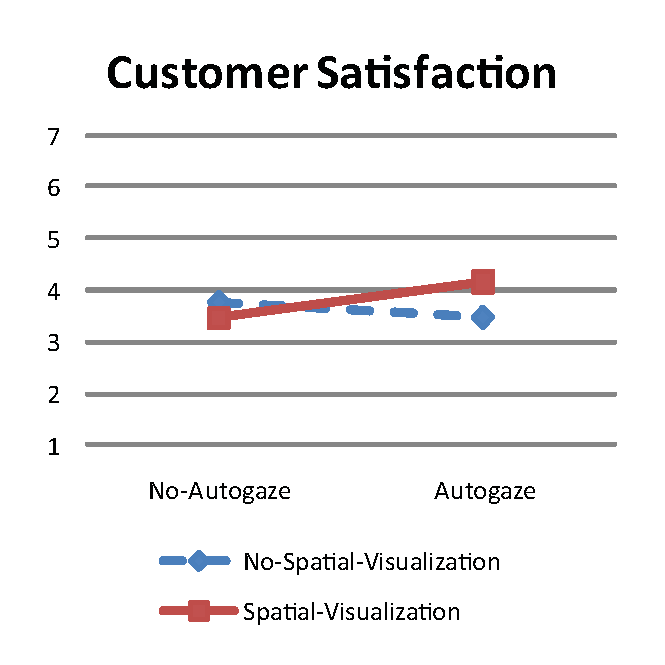
\includegraphics[keepaspectratio, scale= 0.5]{figs/customerSatisfactionFinal2}
		\includegraphics[keepaspectratio, scale= 0.5]{figs/nasaTlxFinal}
		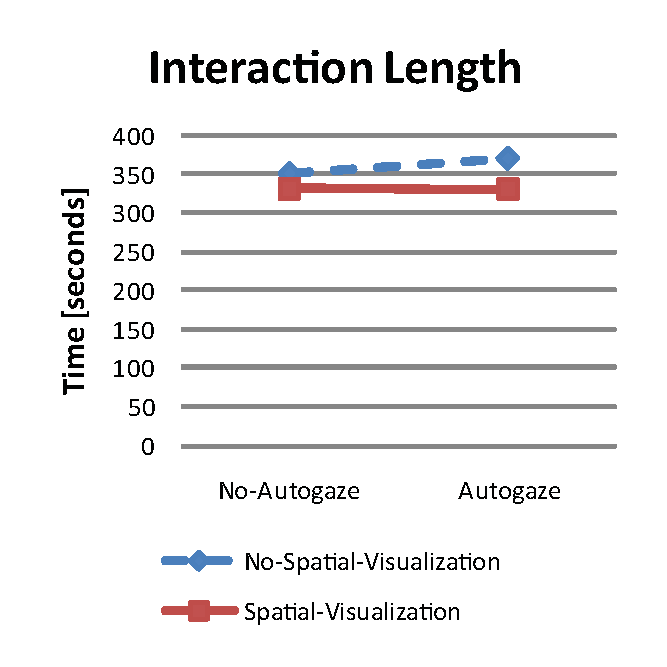
\includegraphics[keepaspectratio, scale=0.5]{figs/interactionLengthFinal}
		\caption{Customer Satisfaction(left), NASA-TLX(center) and Interaction Length(right) }
	\label{fig:results}
\end{figure*}

\subsubsection{Customer's Role}
The customer was instructed to walk into the watch shop and wander around until the robot approaches him/her. 
There is no scripted conversation; instead, the customer is given a situation and a watch that should be the target one. 
An example of a situation is that the customer will participate in a wedding and is interested in buying a watch. 
The customer is also instructed to wait until at least 3 different watches have been presented to make a purchase. 
If none of the watches that have been presented within those 3 watches is the targeted one, the customer will wait until the robot presents this watch and finally purchase it.

\subsection{Conditions}
A $2\times2$ within-subjects experimental design was used with the following conditions: 
\begin{itemize}
	\item {\bf Visualization of Spatial Relationships} factor
		\begin{itemize}
			\item[$\circ$] No-Spatial-Visualization; in this condition, only the URG laser sensor raw data are shown, along with a 3D model of the robot, and the video feed coming from one of the robot's cameras. 
			\item[$\circ$] Spatial-Visualization; this condition adds 3D models of the objects (static, located in the room) and also avatar(s) of the persons (customers, keeping track of their current location).
		\end{itemize}
	\item {\bf Automatic Gaze Control} factor
		\begin{itemize}
			\item[$\circ$] Autogaze; in this condition, a button enables the automatic tracking of the customers. 
			This can be turned off by either pressing the button again, or manually moving the robot's head (via the GUI).
			\item[$\circ$] No-Autogaze; in this condition, the button is disabled, and the only way to control the robot's gaze (presumably to track and observe the customer) is direct manual control via the GUI. 
	\end{itemize}
\end{itemize}

\subsection{Hypothesis and Prediction}
\label{sec:hypothesis}
During a preliminary study, it was observed that an operator had problems carrying out simple interactions due to the overwhelming workload that following a person and observing the person's face presented. 
An automatic control that would allow the system help the operator was implemented, however it was also observed that this solution had repercussions on the awareness of the operator, specifically on the location of the robot with respect to objects in the environment.

It is expected that the proposed automatic gaze control by itself would not contribute to reduce the operator's workload and improve the customer's satisfaction.
However, if the proposed automatic gaze control is combined with an appropriate representation of the spatial relationships of the environment, a positive effect should be observed on the reduction of the operator's workload and the improvement of the customer's satisfaction.
% The proposed automatic gaze control and the 3D representation of spatial relationships are expected to complement each other.
% The utilization of autonomy to handle the robot's gaze control, should reduce the operator's workload and reduce the possibility that the operator will lose track of the customer's face and not see expressions.
% The customer satisfaction should increase due to an improved navigation combined with a better positioning of the robot with respect to objects and humans and a faster reaction time during the interaction.
% The representation of spatial relationships should provide the means by which the operator can transition between observing the customer's face and observing what the customer is referring to in the environment not covered by the video.     

% Therefore, the authors expect that having automatic gaze control and having the visualization of spatial relationships would increase operator understanding of customer intention by:
%Therefore, the authors expect that the combination of the proposed automatic gaze control and the visualization of spatial relationships would increase the quality of the human-robot interaction by:
Therefore, the authors expect that providing the operator with the visualization of spatial relationships would complement the proposed automatic gaze control, increasing the quality of the human-robot interaction by:
\begin{itemize}
	\item reducing operator workload,
	\item increasing customer satisfaction, and
	\item decreasing interaction time.
\end{itemize}
The combination of the visualization of spatial relationships factor and the automatic gaze control factor is expected to result in the highest level of customer satisfaction and present the lowest level of workload.
On the other hand, not having either the visualization of spatial relations factor and automatic gaze control factor should result in the lowest level of customer satisfaction and present the highest level of workload.

\subsection{Evaluation}
A combination of subjective and objective techniques were employed to measure the performance of the operators in each condition:
\begin{itemize}
	\item {\bf Customer satisfaction} was evaluated by asking the customers after each condition to score on a 7-point Likert scale ``how satisfactory was the robot's service?''. In this scale, higher values represent higher customer satisfaction.
	\item {\bf The operator's workload} was evaluated using a NASA-TLX test\cite{hart:tlx} that the operator had to complete after each condition. The result of this test is in a range between 0 and 100 points. Lower values represent lower workload, whereas higher values represent higher workload. In the context of this study, lower workload represents a more focused, efficient operator.
	\item As an indicator of how well the performance of the operator was, the authors timed the total {\bf interaction length} of each condition. In our study, longer interactions are regarded as inefficient since they represent a ``bored'' customer.
\end{itemize}

% \begin{figure*}[t]
% 	\centering
% 	\begin{tabular}{@{}cc@{}}	
% 		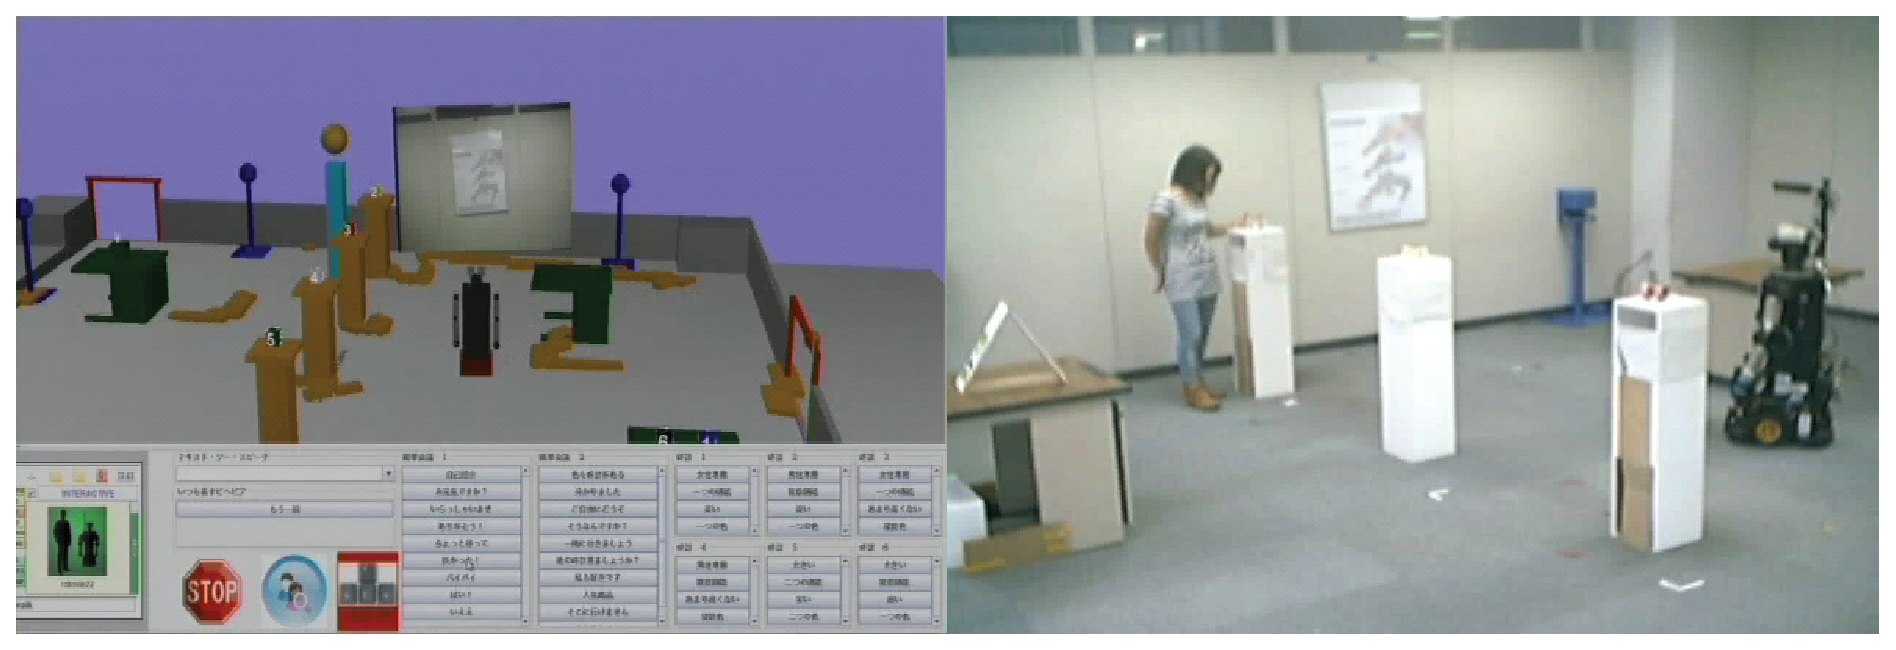
\includegraphics[width=\columnwidth]{figs/opATogether_1} &
% 		\includegraphics[width=\columnwidth]{figs/opATogether_2}\\
% 		a) Operator finds customer by looking at the interface &
% 		b) Robot points correctly to a watch\\
% 		\includegraphics[width=\columnwidth]{figs/opATogether_3} &
% 		\includegraphics[width=\columnwidth]{figs/opATogether_4}\\
% 		c) Operator automatically tracks the customer &
% 		d) Operator observes customer's facial expressions
% 	\end{tabular}
% 		\caption{Natural interaction achieved using visualization and autogaze.}
% 	\label{fig:opATogether}
% \end{figure*}

%%%%%%%%%%%%%%%%%%%%%%%%%%%%%%%%%%%%%%%%%%%%%%%%%%%%%%%%%%%%%%%%%%%%%%%%%%%%%%%%
\section{Results}
%\subsection{Verification of Hypothesis}
\label{sec:verification}
The results presented in Figure~\ref{fig:results} share the following format: the blue dotted series represent the condition No-Spatial-Visualization, the red continuous series correspond to the Spatial-Visualization condition for the spatial relationships factor. 
The $x$-axis represents the ``No-Autogaze'' and ``Autogaze'' conditions corresponding to the experimental factor ``automatic gaze control''. 
A two-way repeated measures Analysis of Variance (ANOVA) was conducted with two within-subject factors, visual relationships and automatic gaze control, for all the results presented in this section. 

\subsection{Customer Satisfaction}
Figure~\ref{fig:results} (left) shows the results corresponding to the customer satisfaction.
No significant main effect was revealed for either the automatic gaze control factor ($F(1,21)=2.094$, $p=.163$, partial $\eta^2=.091$) or the visualization of spatial relationships factor ($F(1,21)=1.817$, $p=.192$, partial $\eta^2=.294$).
The interaction between the visualization of spatial relationships factor and automatic gaze control factor was significant ($F(1,21)=5.431$, $p=.030$, partial $\eta^2=.205$).
The automatic gaze control factor indicated significance for Spatial-Visualization ($p=.003$), however for No-Spatial-Visualization no significant difference was revealed ($p=.367$).
The visualization of spatial relationships factor indicated significance for Autogaze ($p=.015$), however for No-Autogaze no significant difference was revealed ($p=.250$).
%These results show that the factors by themselves did not contribute to increase the customer's satisfaction, however, the combination of visualization of spatial relationships and automatic gaze control positively affected the customer's satisfaction.
These results show that the effect of the ``operator out-of the loop'' problem present while an operator relies in a system's automation was reduced due to the presence of spatial relationships representations in the environment.
These results support our prediction that the proposed automatic gaze control used with our 3D representation of spatial relationships would improve the customer's satisfaction.


%The interaction between the visualization of spatial relationships factor and automatic gaze control factor was significant ($F(1,21)=5.431$, $p=.030$, partial $\eta^2=.205$) as presented in Figure~\ref{fig:results} (left).
%No significant main effect was revealed for either the automatic gaze control factor ($F(1,21)=2.094$, $p=.163$, partial $\eta^2=.091$) or the visualization of spatial relationships factor ($F(1,21)=1.817$, $p=.192$, partial $\eta^2=.294$).
%The automatic gaze control factor indicated significance for Spatial-Visualization ($p=.003$), however for No-Spatial-Visualization no significant difference was revealed ($p=.367$).
%The visualization of spatial relationships factor indicated significance for Autogaze ($p=.015$), however for No-Autogaze no significant difference was revealed ($p=.250$).
%These results support our prediction that the combination of visualization of spatial relationships and automatic gaze control would positively affect the customer's satisfaction. However, the factors by themselves did not contribute to increase the customer's satisfaction.

\subsection{NASA-TLX}
%However, the automatic gaze control factor alone does not support this hypothesis.
The results measured by the NASA-TLX test are depicted in Figure~\ref{fig:results} (center).
A significant main effect was revealed with the visualization of spatial relationships factor ($F(1,21)=14.693$, $p=.001$, partial $\eta^2=.412$) but did not show significance with the automatic gaze control factor ($F(1,21)=.006$, $p=.939$ partial $\eta^2=.000$).
Interaction within these factors was significant ($F(1,21)=4.984$, $p=.037$, partial $\eta^2=.192$).
The visualization of spatial relationships factor revealed a significant effect for Autogaze ($p=.000$) and it also indicated a significant effect for No-Autogaze ($p=.041$).
The automatic gaze control factor did not reveal a significant difference for either No-Spatial-Visualization or Spatial Visualization.
These results demonstrate the importance of providing the operator with a visualization of spatial relationships and that when combined with the proposed automatic gaze control the operator's workload is reduced. 
These results support our prediction that combining the visualization of spatial relationships and automatic gaze control decreases the workload of the operator. 

% The results measured by the NASA-TLX test depicted in Figure~\ref{fig:results} (center), revealed a significant main effect with the visualization of spatial relationships factor ($F(1,21)=14.693$, $p=.001$, partial $\eta^2=.412$) but did not show significance with the automatic gaze control factor ($F(1,21)=.006$, $p=.939$ partial $\eta^2=.000$).
% Interaction within these factors was significant ($F(1,21)=4.984$, $p=.037$, partial $\eta^2=.192$).
% The visualization of spatial relationships factor revealed a significant effect for No-Autogaze ($p=.041$) and it also indicated a significant effect for Autogaze ($p=.000$). 
% The automatic gaze control factor did not reveal a significant difference for either No-Spatial-Visualization or Spatial Visualization. 
% The results confirm our prediction that the combination of visualization of spatial relationships and automatic gaze control decrease the workload of the operator. 
% However, the automatic gaze control factor alone does not support this hypothesis. 

\subsection{Interaction Length}
The results measuring the interaction length are shown in Figure~\ref{fig:results} (right).
A significant main effect was revealed in the visualization of spatial relationships factor ($F(1,21)=8.747$, $p=.008$, partial $\eta^2=.080$).
The interaction between these two factors did not present a significant effect ($F(1,21)=.798$, $p=.382$, partial $\eta^2=.037$).
No significant effect was shown by the automatic gaze control factor ($F(1,21)=1.190$, $p=.288$, partial $\eta^2=.054$).
From these results it can be seen that when the operator was provided with the visualization of spatial relationships, interactions were shorter and more efficient.
%The combination of these two factors did shorten the interaction with the customer.
These results support our hypothesis with respect to the positive effect that the visualization of spatial relationships have in the length of the interaction with a customer. 
%The results support our hypothesis regarding the effect of representing spatial relationships in the length of the interaction, however, the automatic gaze control did not contribute to decrease the interaction length as expected.

% The results depicted in Figure~\ref{fig:results} (right), revealed a significant main effect in the visualization of spatial relationships factor ($F(1,21)=8.747$, $p=.008$, partial $\eta^2=.080$).
% However, no significant effect was shown by the automatic gaze control factor ($F(1,21)=1.190$, $p=.288$, partial $\eta^2=.054$). 
% The interaction between these two factors did not present a significant effect ($F(1,21)=.798$, $p=.382$, partial $\eta^2=.037$). 
% These results support our hypothesis regarding the visualization of spatial relationships, however, the automatic gaze control does not support our prediction.

% \begin{figure*}[t]
% 	\centering
% 	\begin{tabular}{@{}cc@{}}
% 		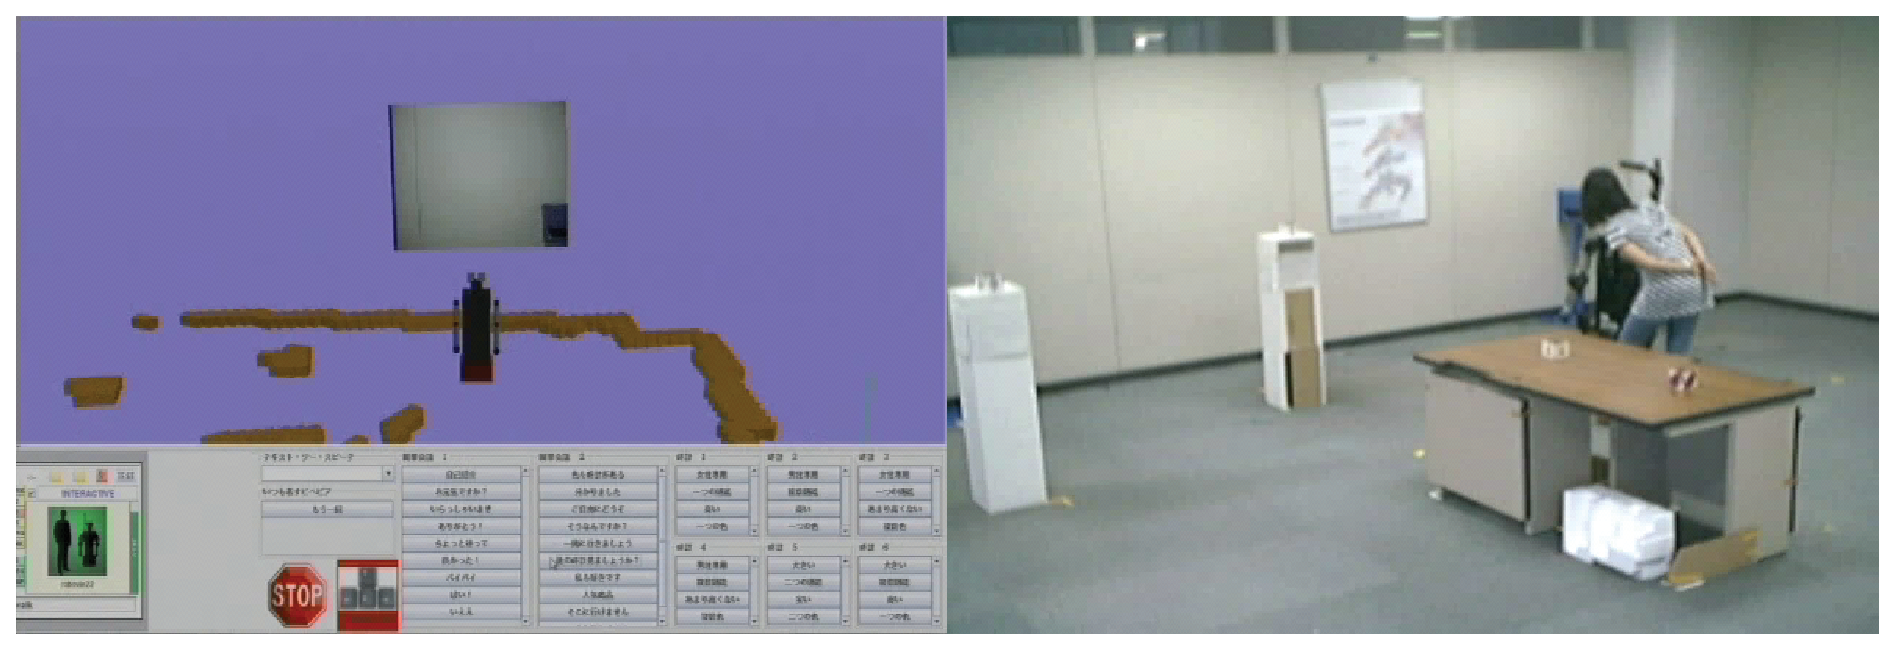
\includegraphics[width=\columnwidth]{figs/nopNaTogether_1} &
% 		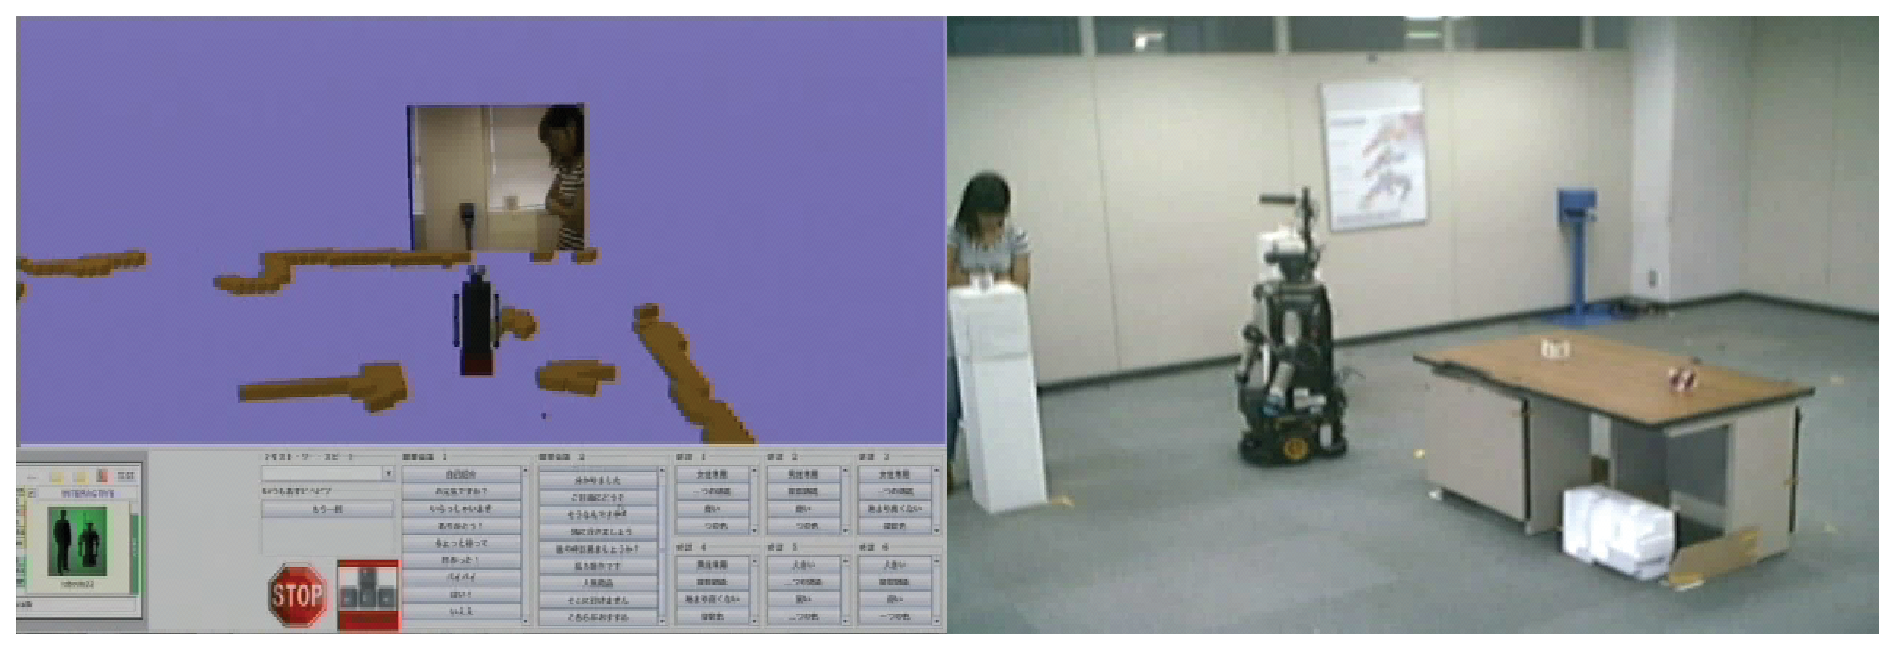
\includegraphics[width=\columnwidth]{figs/nopNaTogether_2}\\
% 		a) Operator looks for the customer &
% 		b) Operator finds the customer and interacts\\ 
% 		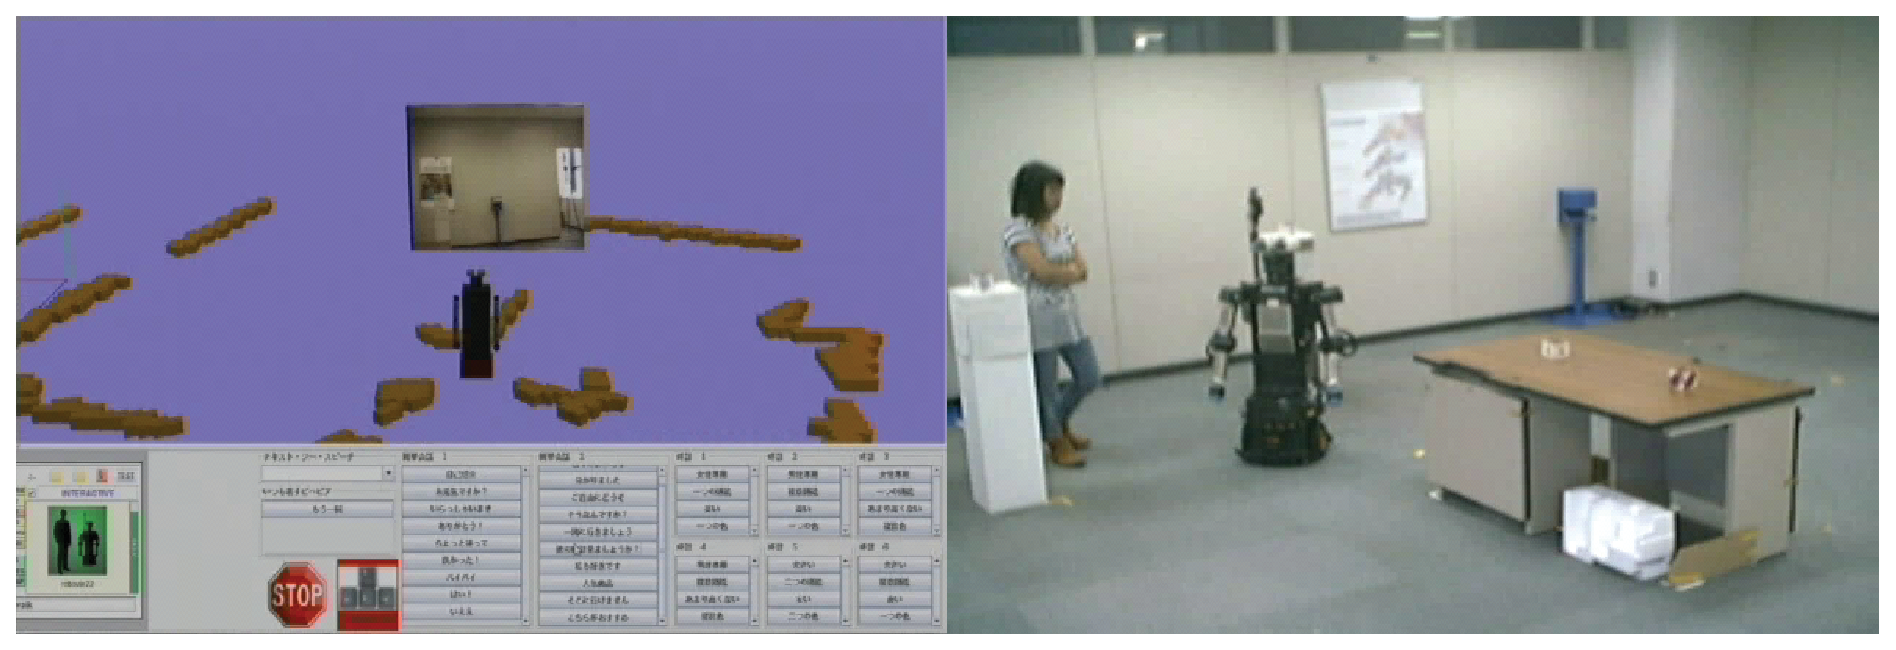
\includegraphics[width=\columnwidth]{figs/nopNaTogether_3} &
% 		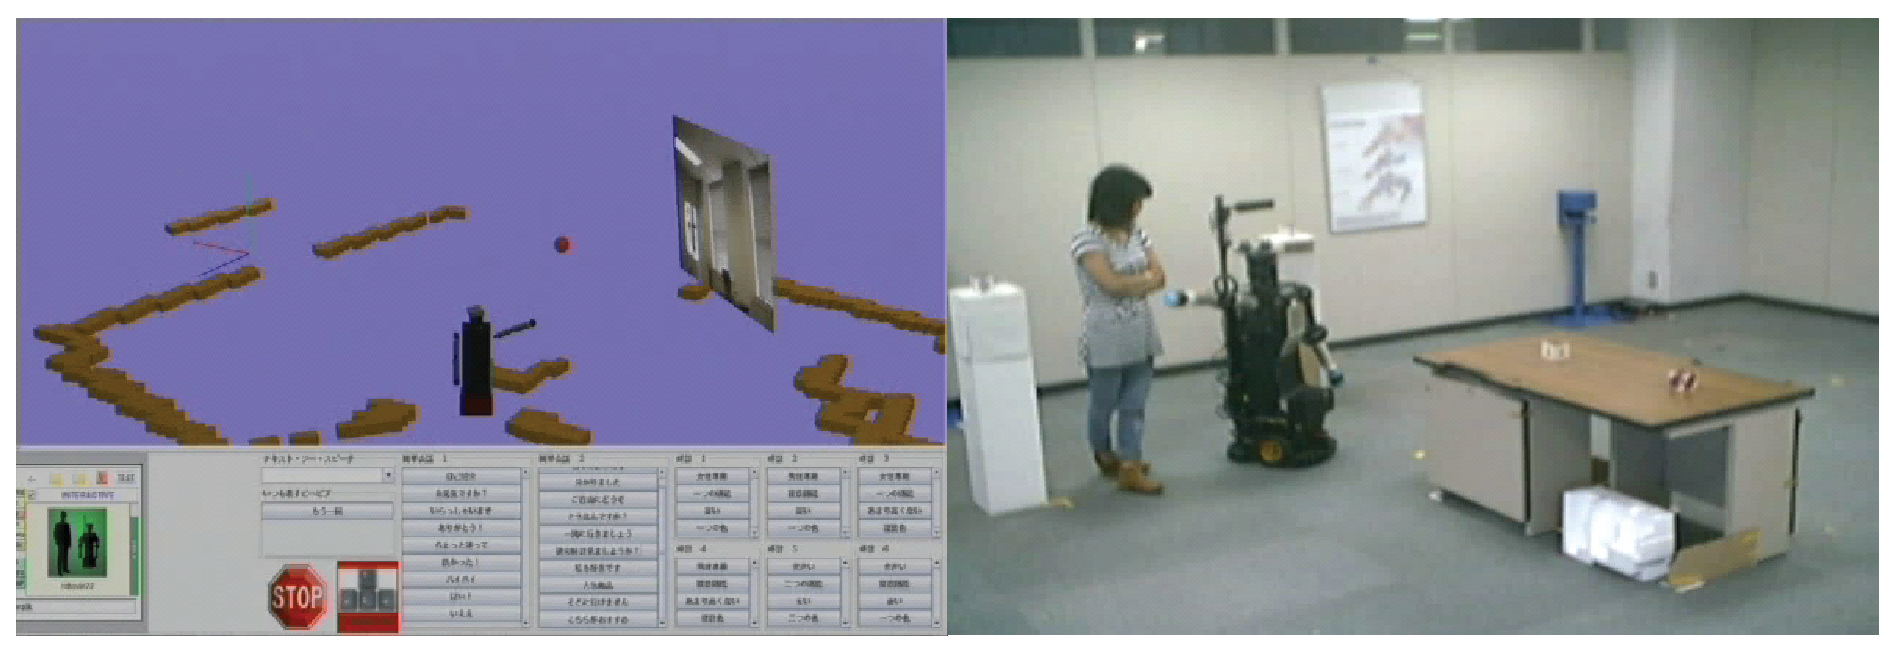
\includegraphics[width=\columnwidth]{figs/nopNaTogether_4}\\
% 		c) Robot spins looking for another watch &
% 		d) Robot points incorrectly and loses the customer
% 	\end{tabular}
% 		\caption{Poor interaction when using no-visualization and no-autogaze.}
% 	\label{fig:nopNaTogether}
% \end{figure*}


These results support our prediction that the representation of spatial relationships and automatic gaze control complement each other and that when combined, they have a positive effect on the customer's satisfaction. 
It was also demonstrated that the factors by themselves did not contribute to increase the customer's satisfaction.

% The fact that the automatic gaze control by itself did not contribute to increase the customer's satisfaction may be due to an absence of an external point of reference from which the operator can understand where the robot is located at any given moment. 
% The operator spends time observing the facial expressions and gestures of the customer and becomes ``used'' to this view. 
% However, when the customer points to another location or asks about an object in another location, the field of view of the camera is insufficient and the operator must look within the 3D environment for the corresponding desired location. 
% If the operator is not provided with an appropriate representation of the spatial relationships of the environment, the operator must remember were the desired object's location is, confirm its location by looking at it and finally, while navigating towards the target location, use the robot's camera to avoid collisions.
% This increased effort translates in longer interactions and ``unnatural'' interaction with the customer. 
% Therefore, while it is important to alleviate the operator's workload by introducing shared autonomy in the teleoperation system, it is essential to provide, at the same time, the operator with the tools to understand the spatial relationships governing the environment where the robot is located.
%It can be concluded that, while it is important to alleviate the operator's workload by introducing shared autonomy in the teleoperation system, it is essential to provide, at the same time, the operator with the tools to understand the spatial relationships governing the environment where the robot is located.
%It can be concluded that, while it is important to alleviate the operator's performance by introducing shared autonomy in the teleoperation system, it is essential to provide, at the same time, the operator with the tools to understand the spatial relationships governing the environment where the robot is located.
It can be concluded that, while increasing the autonomy of the system is effective in reducing the operator’s workload, it is essential to provide, at the same time, the operator with the tools to understand the spatial relationships governing the environment where the robot is located.


% \subsection{Observations}
% The authors present two interaction examples in this section; one without visualization of spatial relationships or automatic gaze control, and one with both.
% These examples present an insight on how operators teleoperated the robot under different conditions and the effect of these conditions on their performance. 
% 
% \subsubsection{Case 1: With visualization and with autogaze}
% This case (Figure~\ref{fig:opATogether}), serves as an example of a smooth interaction.
% The operator having an understanding of where objects are in the environment and allowing the robot to track the customer, is able to take an initiative in the interaction by showing the customer a watch in another location. 
% A transcript of this continuous interaction is given as follows (where, Robot $=$ R and Customer $=$ C):
% \begin{itemize}
% 	\item[] {\bf R:} Operator finds the customer just by looking at her 3D representation. ``One moment please''.
% 	\item[] {\bf R:} ``Are you looking for something?''  (Figure~\ref{fig:opATogether}(a))
% 	\item[] {\bf Customer:} ``Yes, I'm looking for a watch to give as a present''.
% 	\item[]	{\bf R:} Robot moves towards a watch and faces it. ``I see.'' 
% 	\item[] {\bf R:} Pointing correctly to the watch, ``How about this one?'' (Figure~\ref{fig:opATogether}(b))
% 	\item[] {\bf C:} Operator enables automatic gaze control to observe the customer's facial expressions, Customer moves towards the watch. ``This one, huh?'' (Figure~\ref{fig:opATogether}(c))
% 	\item[] {\bf R:} While looking at customer's face. ``I would recommend this one''. (Figure~\ref{fig:opATogether}(d))
% \end{itemize}
% 
% The operator can differentiate a stand or a watch from a person only by looking at their respective visualizations as 3D models.
% This case illustrates that the this visualization in combination with the automatic gaze control allows the operator to react faster, improving the customer satisfaction and decreasing the operator's workload (as shown in the results presented in Section~\ref{subsubsec:verification}.
% 
% \subsubsection{Case 2: Without visualization and without autogaze}
% When the operator has limited understanding of the location of objects in the environment spends more time looking for them through the use of the robot's camera.
% This additional actuation task forces the operator to manually control the robot which may produce awkward social behaviors.
% A transcript of this continuous interaction presented in Figure~\ref{fig:nopNaTogether} is shown:
% \begin{itemize}
% 	\item[] {\bf R:} Operator tries to find the customer spinning the robot Figure~\ref{fig:nopNaTogether}(a).
% 	\item[] {\bf C:} Looks at the robot to try to understand its intention.
% 	\item[] {\bf R:} After a long pause the operator finally finds the intended watch. ``How about these one?''. Figure~\ref{fig:nopNaTogether}(b).
% 	\item[]	{\bf C:} Looks at the watch.
% 	\item[] {\bf R:} ``This watch has many functions. It comes in one color''. 
% 	\item[] {\bf C:} ``Really?'' 
% 	\item[] {\bf R:} Operator tries to look at customer's face. ``I like it. Do you want to see another watch?''
% 	\item[] {\bf C:} ``Yes''.
% 	\item[] {\bf R:} Operator looks around, apparently confused, by spinning the robot. Figure~\ref{fig:nopNaTogether}(c)
% 	\item[] {\bf R:} Pointing to an incorrect location. ``How about that one?''.
% 	\item[] {\bf C:} Does not know which watch the robot talks about, long pause. Asks for confirmation. ``This one?'' Figure~\ref{fig:nopNaTogether}(d).
% \end{itemize}
% When there is lack of a visualization of the objects in the environment, the operator relies on the video feed in order to understand where static or dynamic objects are. 
% This makes the operator look for these objects by spinning the robot, which can translate into a socially awkward behavior. 
% As presented in Section~\ref{subsubsec:verification}, this affects negatively the performance of the operator since it increases the operator's workload. 


%%%%%%%%%%%%%%%%%%%%%%%%%%%%%%%%%%%%%%%%%%%%%%%%%%%%%%%%%%%%%%%%%%%%%%%%%%%%%%%%
\section{Discussion}

\subsection{Summary}
The results of our study indicate that when: a) an operator has an understanding of the spatial relationships, and b) the level of actuation the operator has to perform is decreased through automation of necessary and/or routine tasks, the operator can focus more on the overall task. 
In our setting, the visualization of where the persons and the objects are, combined with automatic gaze control that frees the operator from tracking the person in order to observe them and thus determine their intentions, has resulted in improved customer satisfaction, that could be related to the reduced operator workload. 
However, it was observed that the automation of the gaze, by itself, did not enhance the customer satisfaction. 
Therefore, the authors would argue towards an approach in teleoperation architecture design that incorporates both the visualization of spatial relationships and the automation of processes that are necessary within an HRI context to aid the operator in improving their understanding of human non-verbal communication and which are crucial for social interactions.
This approach has applications both for teleoperated systems (for improving the operator performance), but also for research towards fully-automated systems, as first steps towards understanding the requirements necessary to implement the social processes to be automated (such as the automatic gaze control in our current work). 

\subsection{Limitations}
In our current work, the robot can keep track of a single person within its field of view. 
However, it is conceivable that in a different social context, the robot would have to interact with multiple people at the same location (e.g.\ guiding a crowd at a museum).
In the future, this could be augmented by additional mechanisms that e.g.\ automatically determine the gaze of the person or any pointing gestures. 
The visualization of spatial relationships currently relies on \emph{a priori} knowledge of a static environment, as well as the existence of environmental sensors.
Both of these limitations may be addressed by using traditional robot navigational and localization techniques and also by relying on on-board sensors.
%In both cases, the desired accuracy would determine the trade-off between using a specific solution.
 
%%%%%%%%%%%%%%%%%%%%%%%%%%%%%%%%%%%%%%%%%%%%%%%%%%%%%%%%%%%%%%%%%%%%%%%%%%%%%%%%
\section{Acknowledgments}
The authors would like to acknowledge Florent Ferreri, Kyle Sama for their invaluable help on the development of the proposed system and the experiment carried out and presented in this paper. 
This research was supported by the Ministry of Internal Affairs and Communications of Japan.

%%%%%%%%%%%%%%%%%%%%%%%%%%%%%%%%%%%%%%%%%%%%%%%%%%%%%%%%%%%%%%%%%%%%%%%%%%%%%%%%
\bibliographystyle{abbrv}
\bibliography{moraIROS2011}

%\balancecolumns
% That's all folks!
\end{document}

\end{document}